\newthought{\textbf{Jihan Dwi Sarah - 2020903430015 - TRKJ 3B}}


\newday{\textbf{1 Desember 2022}}
\begin{enumerate}
\item Kendala dan Solusi
% jelaskan kendala dan penyebab yang dialami saat mengikuti praktikum serta solusi atau langkah-langkah yang telah dilakukan
\begin{itemize}
\item Praktikum pertama yaitu melakukan pull dan push Github. Selama praktikum tidak ada kendala. Yang dilakukan selama praktikum pertama yaitu mengedit file pada Latex yaitu menambahkan asal sekolah dan tempat tinggal.
\item Praktikum selanjutnya tidak ada kendala. Yang dilakukan selama praktikum adalah mengganti nama beserta NIM di Latex pada halaman laporan praktikum masing-masing.
\end{itemize}

\item Kesimpulan
% berikan kesimpulan dari praktikum yang telah dikerjkan
\begin{itemize}
\item Berhasil melakukan pull dan push menggunakan Github. 
\item Berhasil mengganti nama beserta NIM pada halam laporan.
\end{itemize}
\end{enumerate}


\newday{\textbf{2 Desember 2022}}
\begin{enumerate}
\item Kendala dan Solusi
% jelaskan kendala dan penyebab yang dialami saat mengikuti praktikum serta solusi atau langkah-langkah yang telah dilakukan
\newline Praktikum selanjutnya tidak ada kendala. Yang dilakukan selama praktikum adalah membuat laporan praktikum serta menambahkan baris baru untuk tiap-tiap tanggal pelaksanaan praktikum.

\item Kesimpulan
% berikan kesimpulan dari praktikum yang telah dikerjkan
\newline Berhasil mengedit halaman laporan praktikum.
\end{enumerate}


\newday{\textbf{8 Desember 2022}}
\begin{enumerate}
\item Kendala dan Solusi
% jelaskan kendala dan penyebab yang dialami saat mengikuti praktikum serta solusi atau langkah-langkah yang telah dilakukan
\newline Pada pertemuan hari ini, kegiatan yang dilakukan adalah menginstall Apache Hadoop. Selama praktikum tidak mengalami kendala.

\item Kesimpulan \\
% berikan kesimpulan dari praktikum yang telah dikerjkan
Berhasil melakukan instalasi java tanpa ada bug atau error serta instalasi hadoop berikut ini gambar hasil verifikasi instalasi java version dan hadoop version 

\begin{figure}[!ht]
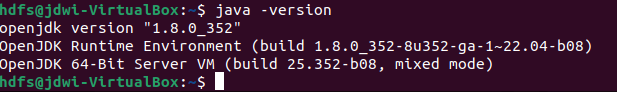
\includegraphics[width=\textwidth]{JihanDwiSarah/Java-version(Jihan)}
\caption{Verifikasi Hasil Instalasi Java}
\label{gam:Java-version(Jihan)}
\end{figure} 

\begin{figure}[!ht]
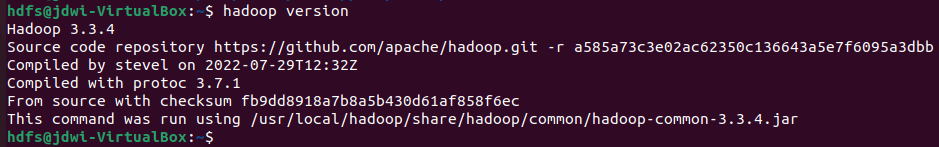
\includegraphics[width=\textwidth]{JihanDwiSarah/Hadoop-version(Jihan)}
\caption{Verifikasi Hasil Instalasi Hadoop}
\label{gam:Hadoop-version(Jihan)}
\end{figure}
\end{enumerate}


\newday{\textbf{9 Desember 2022}}
\begin{enumerate}
\item Kendala dan Solusi \\
% jelaskan kendala dan penyebab yang dialami saat mengikuti praktikum serta solusi atau langkah-langkah yang telah dilakukan
Pada pertemuan hari ini, kegiatan yang dilakukan adalah mengkonfigurasi Apache Hadoop. Selama praktikum tidak mengalami kendala.

\item Kesimpulan \\
% berikan kesimpulan dari praktikum yang telah dikerjkan
Berhasil mengkonfigurasi beberapa file Hadoop sehingga memudahkan dalam memonitoring ekosistem Hadoop yang telah diinstall. Berikut ini gambar bukti keberhasilan praktikum. 

\begin{figure}[!ht]
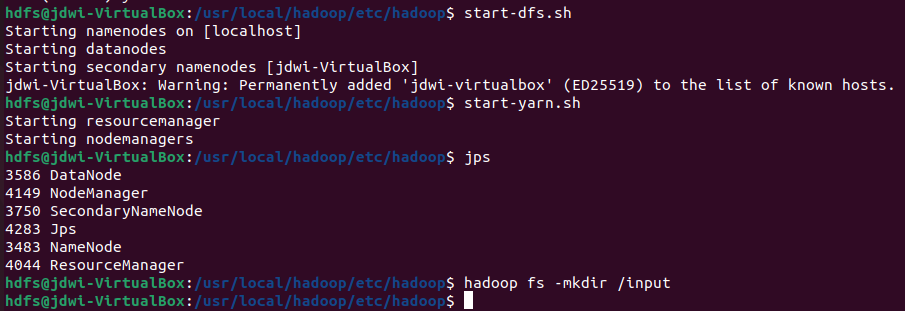
\includegraphics[width=\textwidth]{JihanDwiSarah/perintah-jps(jihan)}
\caption{Hasil perintah jps}
\label{gam:perintah-jps(jihan)}
\end{figure} 

\vspace*{-1cm}
\begin{figure}[!ht]
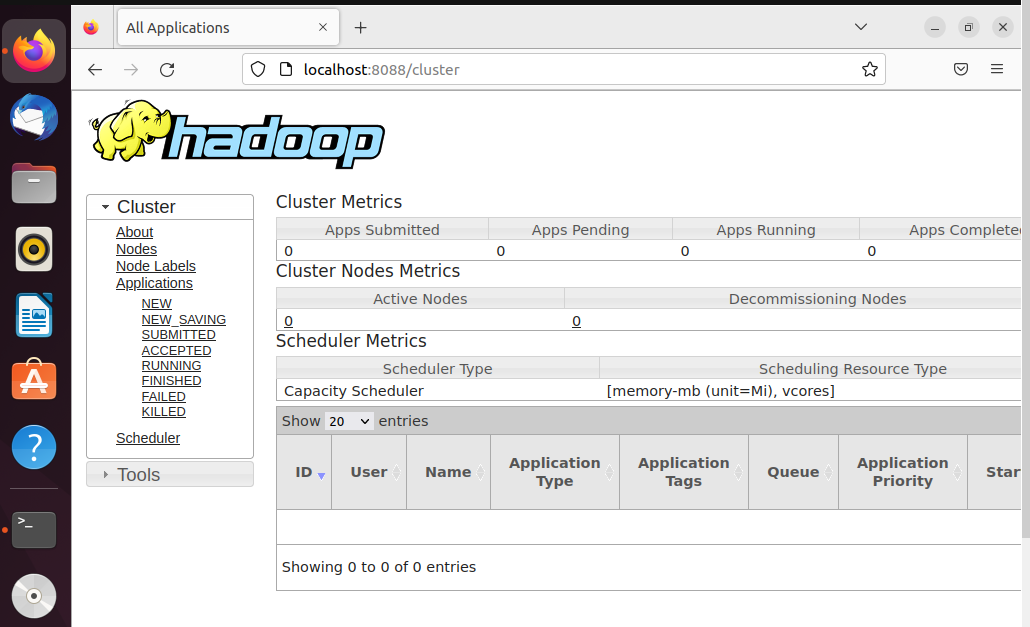
\includegraphics[width=.85\textwidth]{JihanDwiSarah/Akses-web-browser-8088(Jihan)}
\caption{Akses melalui web browser dengan alamat http://localhost:8088}
\label{gam:Akses-web-browser-8088(Jihan)}
\end{figure} 

\vspace*{-1cm}
\begin{figure}[!ht]
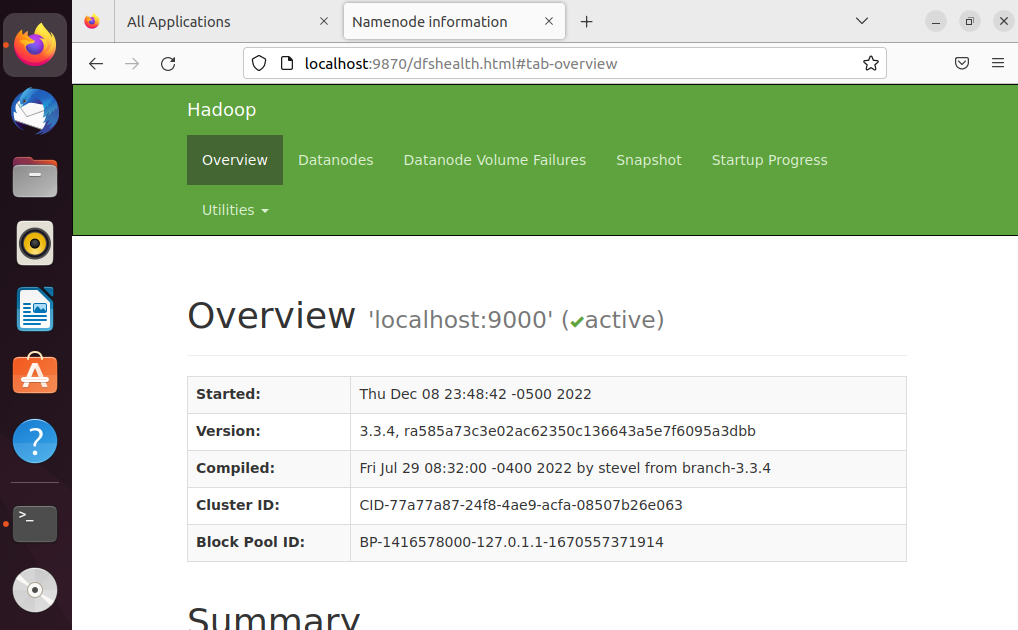
\includegraphics[width=.85\textwidth]{JihanDwiSarah/Akses-web-browser-9870(Jihan)}
\caption{Akses melalui web browser dengan alamat http://localhost:9870}
\label{gam:Akses-web-browser-9870(Jihan)}
\end{figure} 
\end{enumerate}